\chapter{Theory}
	
\section{Reference systems}
	Reference systems is an important part of analysis of moving dynamical systems. When one derive the motion of 
	a system one will need some reference fram to calculate the motion relative too. There are a couple of different 
	reference systems used today. One is the ECEF-frame (Earth-Centered, Earth-Fixed), which has the center of the 
	earth as the origin of the frame. The frame rotates with the earth, but when the speed of the vessel is low, 
	this frame can be considered inertial. \cite{forsell}
	
	Another common reference frame are the NED frame (North-East-Down). It is defined as the tangetial plane at 
	the earth's surface moving with the vessel. It assumes that the Earth's rotation can be neglected, and this means 
	that frame is not valid for inter-continental travel, because it is not strictly inertial. It is defined with 
	the x-axis pointing towards the Earth's true north, the y-axis pointing towards the east, and the z-axis 
	pointing downwards toward Earth's center. The NED-frame is defined relative to the ECEF-frame by the means of 
	two angles, \textit{longitude} and \textit{latitude}. This is the global reference system that will be used 
	in this report. \cite{fossen}
	
	The last reference system used is the Body-frame, which all forces, moments, linear velocities and angular 
	velocities will be expressed in. This frame has it's center in the Center of Gravitiy (CG) of the vessel. The 
	x-axis is defined in the logitudinal axis of the vessel, y-axis to the right, and the z-axis is directed 
	downwards to complete the right hand-system. The body-frame values are transformed to the NED-frame by the means 
	of a Rotataion matrix.
	
	
	

\section{Hydrodynamic Model}
	\label{sec:ch1-model}
	An Autonomous Underwater Vehicle is a complex, non-linear and coupled process. The model which is used in this
	report uses the 6 DOF model described in \cite{fossen}.
	\begin{equation}
	\label{eq:ch1-model}
		\begin{aligned}
			\mathbf{\dot{\eta}} &= \rotation \mathbf{\nu} \\
			\mass + \coriolis + \damping + \restoring &= \force \\
		\end{aligned}
	\end{equation}
	The Equation \eqref{eq:ch1-model} describes the kinematics and kinetics for the model. It is in the 
	mathematical sense just a Mass-damper-spring system. The coriolis term, $\mathbf{C}(\mathbf{\nu})$, is 
	a skew-symmetric matrix.
	
	The $\rotation$ matrix is the rotation matrix of euler coordinates which relates the velocity of the 
	vessel to actual movment in the global reference system.




\section{Camera therory}
	\label{ch1-cameramodel}
	Using camera for control is not a stright forward problem. Calculations are needed to relate the data discovered 
	by the camera to the real world which the vessel is opperating in. This imply that coordinates of a 2D point in 
	the camera have to be transformed into a 3D point which can be used by the control system onboard the AUV. Since 
	we are going from less knowledge about a point to more knowledge about a point, some things are needed to be 
	estimated or measured to gain the ability to solve the 2D to 3D problem exactely.
	
	The camera properties or parameters can be devided into two cathegories; the intrinsic parameters and extrinsic 
	parameters. The intrinsic parameters are constant parameters and vary from camera to camera. It is the focus 
	distance and image distortion of the pixels away from the center of the camera. The extrincic parameters relate 
	the position of the point relative to camera coordinates. These parameters are ofcourse dependant on the 
	position of the camera and change with time. \cite{robotbok}
	
	
	Suppose a point in the world reference system, denoted by, $P_w \in \mathbb{R}^3$. The same point
	represented in the camera frame, $P_c$ are related to $P_w$ by a rotation matrix, $\mathbf{R} \in
	SO(3)$. This gives the following equation: 
	\begin{equation}
		P_w = \mathbf{R} P_c + O(t)
	\end{equation}
	where $O(t)$ is the origin of the camera frame. This means that the point in the camera view is
	descirbed by the equation
	\begin{equation}
		\label{eq:ch1-P_c}
		P_c = \mathbf{R}^T (P_w - O(t))
	\end{equation}

	A pinhole camera model are used to capture $P_c$ to image coordinates, $P_i \in
	\mathbb{R}^2$. 
	The principle behind a pinehole camera is that all lightbeams passes through a
	infinitesmall hole, or point, located in the origin of the camera frame.   
	\begin{figure}[hbtp]
		\centering
		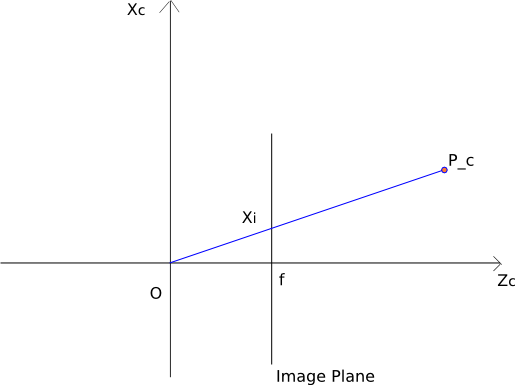
\includegraphics[width=0.7\textwidth]{pics/pinhole_model2}
		\caption{Pinhole Camera Model}
		\label{fig:ch1-pinhole}
	\end{figure}
			
	As seen from Figure \ref{fig:ch1-pinhole} the image plane is located a distance $f$ from the image plane. 
	The point is projected through the hole an onto the image plane. The principal axis of the camere is located in the
	direction of the observed point. For simplicity the image plane are located in the front of the
	pinhole, this is just in theory and is not possible in real camera application. From this the
	perspective equations are derived. \cite{robotbok}
	\begin{equation}
		\label{eq:ch1-perspective}
		P_i = \left[ \begin{array}{cc}
					\frac{f}{z_c} & 0 \\
					0	& \frac{f}{z_c} 
				\end{array} \right] 
				\left[ \begin{array}{c}
					x_c \\
					y_c
					\end{array} \right]
	\end{equation}
	This are the perspective equations which gives the observed point in screen cooridnates. 

\section{Kalman filter}
	Kalman filtering a powerful and versatile tool in estimation and sensor fusion. A Kalman filter is
	usually employd in navigation applications to fuse GPS and INS together. By this way one will have
	the speed and resolution of an INS system and the precission of the GPS system.
	

	The Kalman Filter is as stated befor a very versatile tool which can be employed allmost in
	any application. The downside with the Kalman filter is that it is a Linear system, and can only
	guarantee optimality for linear systems. The system considered in this report is nonlinear and one can not
	use the Kalman filter directly on this system. There is a nonlinear version of the Kalman filter, the
	Extended Kalman Filter, which uses the same assumptions as the linear version but uses the nonlinear
	model to predict the state forward. When updating the Covariance matrix the system equations are
	linearized around the current estimate and updated according to certain update laws. This introduces some
	significant problems. First the filter might converge towards wrong values, because of a non-positive-definite
	covariance matrix. This is mostly due to poor linearization of the state equations. \cite{kalman}
	
\section{Guidance Algorithms}
        \label{chap1-guidance-alg}
        The guidance algorithm is one of the most important part of an autonomous vehicles control system. It
	needs to be robust and be able to handle moast situations. A guidance system should be able to give
	feasible commands to the lower level control system which controls the actuators, and should be able
	to handle most situations with care. The guidance system should decide the best trajectory to be
	followed based on the target location and physical capabilities of the system.\cite{GuidanceReview}

	Most of the guidance algorithms originates from airborne missile systems. This have been well
	documented and proven to work in numerous cases. Common guidance scheems such as Line-of-sight (LOS)
	and Proportional Navigation Guidance (PNG) and vareious implementations of these are employed in
	numerous guidance systems.
	
		\begin{figure}[hbtp]
		\centering
		\includegraphics[width=0.83\textwidth]{pics/waypoint}
		\caption{Variables assosiated with path following}
		\label{fig:ch2-pathfollowing}
	\end{figure}
	The Figure \ref{fig:ch2-pathfollowing} shows the variables which are important for linear path following. The
	cross-track error, $e$ are an important aspect here. It is the lateral position error decomposed in
	the desired path reference frame. Another variable worth noting is $\Delta$ which is the look-ahead
	distance. This is analogus to when you drive a car you look farther down the road to better maneuver
	the car. A great look-ahead distance yealds smooth heading reference but slower convergence of the
	cross-track error. A lower look-ahead distance gives an agressive heading reference and fast
	convergence of the cross-track error. The $s$-variable are called the along-track distance from point
	$P_k$. 
	
	
	\subsection{Line-of-Sight Guidance Law}
	        Line-of-sight-guidance are the most common principle used. The LOS-algorithm computes
		the line-of-sight angle from the present location to the target location, and uses this
		angle as a reference heading.

		The LOS-angle is fed directly into the 
		heading controller as a reference. When ocean currents and disturbances are present, a
		modified guidance law is presented. This uses the Side Slip angle, defined as:
		\begin{equation}
			\label{eq:ch2-sideslip}
			\beta = \sin^{-1} ( \frac{v}{\sqrt{u^2 + v^2 + w^2}})
		\end{equation}
		The new heading reference is then taken as
		\begin{equation}
			\label{eq:ch2-los-law}
			\psi_d = \psi_{LOS} - \beta
		\end{equation}
		Where $\psi_{LOS}$ is the LOS-angle from the current position to the next waypoint. 

	\subsection{Radius-based Guidance}
		Radius-based guidance uses the point where the radius around the current location intersects
		with the path, denoted on Figure \ref{fig:ch2-pathfollowing} as $P_{int}$. This
		means assigning the desired heading as 
		\begin{equation}
			\psi_d = \tan^{-1}(\frac{y_{int} - y}{x_{int} - y})
		\end{equation}
		where 
		\begin{equation}
			(x_{int} - x)^2 + (y_{int} - y)^2 = r^2
		\end{equation}
		If $r$ is chosen sufficiently large the equations above will have a solution, i.e $r > |e|$
		otherwise there will exist no intersection point on the track line.
		\cite{guidance_planar_path}
	
	\subsection{Lookahead-based Guidance}
		Here the lookahead distance are utilized when calculating the desired heading. If $\psi_d$ are
		chosen as:
		\begin{equation}
			\psi_d = \alpha_k + \psi_r
		\end{equation}
		where $\alpha_k$ is the angle of the path and
		\begin{equation}
			\psi_r = \tan^{-1} (\frac{-e}{\Delta})
		\end{equation}
		By choosing $\psi_r$ in this way the heading is always directed towards the lookahead point at
		the path. It is then easily seen that the cross-track error will converge to zero. This
		method is easier and less computationally intensive than the previously stated Radius-based
		guidance. \cite{guidance_planar_path}

		This method are implemented in the guidance system, because of it simplicity and robustness.
		This method are chosen because pipelines are mostly made up of linear segments. 

	
	\subsection{Proportional Navigation}
		Proportional Navigation Guidance is more effective that LOS-guidance in case of a
		non-maneuvering
		target. It gives less interception time than LOS. The PNG-law can be stated as the following:
		\cite{GuidanceReview}
		\begin{equation}
			\eta_c = N' V_c \dot{\lambda}
		\end{equation}
		where $\eta_c$ is the acceleration command, $N'$ is the navigation ratio, $V_c$ is the closing
		velocity, and $\dot{\lambda}$ is the line of sight angular velocity. The navigation ratio is a
		tuning
		parameter which will give higher demanded acceleration and therby reacing the target in less
		time.

        	The guidance laws mentioned above does not work so well with maneuvering targets and lots of
		solutions have been proposed to make these laws more effective when dealing with moving
		targets. In this case the targets will be non-moving waypoints and the maneuvering laws
		will not be discussed here.
	
	
	\subsection{Various Guidance Concepts}
		A unified path following controller are derived in \cite{control-concept-AUV}. The 
		authors proposes a singel control structure which will work for the entire velocity regiem.
		The controller is derived using backstepping. The concept are shown to be Uniform Global
		Expontially Stable under some assumptions about the guidance signals. The controller will not
		work without properly generated references. The AUV concidered here are fully actuated for low
		speeds but becomes undeactuated for higher speeds. The controller guarantees that the AUV
		converges towards the desired path regardless of if it is underactuated or fully actuated.
		
		In \cite{optimal-cross-track} an optimal cross-track guidance scheme are proposed. It seeks to minimize
		the crosstrack-error, depth, pitch and yaw by using the pitch rate and yaw rate, this is called Model
		Predictive Guidance. Damping and can be added to reduce the commanded pitch and yaw rates which can
		cause overshoot. The guidance scheme are compared against a LOS guidance system and gives good
		results.

	
\section{Different Methods for Pipeline Following Discussed in Literture}
	A literature study was performed to see what other people have acomplished on the subject on AUV and 
	pipeline following. 

	\cite{piscis} describes breefly a prototype AUV equipped with a camera and sonar to carry out pipeline
	inspection missions. The AUV uses controllers for heading, speed and depth and visual guidance to
	follow the pipeline. 
	
	\cite{GuidanceReview} proposes a 2-stage guidance problem. When submerging and ascending to the surface, 
	the AUV uses a LOS guidance law at full speed. When the pipeline is aqcuired the guidacen law is switched 
	to a visual guidance scheem, which allows for a precise guidance over the subsea cable or pipeline. 
		
	In \cite{MPC_pure_pursuit} a guidance system using Model Predictive Control (MPC) and PNG law was used to make 
	a guidance system able to track cables and pipelines on the sea bed using Doppler Velocity Log and Electro-
	Magnetic sensors to find the cable/pipeline. The report utilizes the pure pursuit scheeme, similiar to what 
	predadtors do when they are hunting the pray. The cable/pipeline and AUV is formulated as moving points with 
	mass. The engages in a tail chase with the pipeline ``point``, but the AUV never catches up with it. This 
	method is robust to model uncertanties and handles constraints of the vessel in a systematic way. The controller
	however shows problems when a current is introduced in the system. The AUV drifts of the pipeline, but catches 
	up with the waypoints in the end.
	
	In \cite{Visual_inpsection_of_seabottom_by_AUV} a visual guidance system for inspection of undewater structures 
	is presented. The visual system uses an Extended Kalman Filter to smooth and predict where the structure i.e. 
	pipeline will move in the next sample interval of for the image processing software. A 3 dimentional model 
	of the scene is constructed which then allows the guidance sytem to calculate an input to the controllers.
	
	\cite{reactive_control_AUV} proposes a reactive control approach to pipeline tracking together with a 
	profiling sonar. Reactive control originated from the field of obstacle avoidance in autonomous land and air 
	vehicles. It uses \textit{Deformed Virtual Zones} (DVZ) which describes the interaction between the AUV and 
	the pipeline. The controller tries to minimize the defromation of the DVZ and calculates a feasible control input. 
	The DVZ in this case is a prism with a cylidrical cavity directly underneth the AUV. If the AUV moves away from 
	the pipeline the DVZ will be deformed and the controller will try to counteract the motion. This is a 
	computational inexpensive way of achieving a good pipeline following. This method shows promising results 
	but has yet to be implemented and tested in real-life scenarios. 
	
	In \cite{fuel_optimal_control} a fuel-optimal tracking controller is derived to minimalize the fuel consumption 
	of the AUV. It uses the fact that the least fuel consuming path is the shortest one. This
	paper deives a fuel optimal controller using the estimated fuel consumption as a minimization index. 

	\cite{side_scan_sonar} describes two technices for detecting and tracking pipelines using Side Scan
	Sonar and Multi-Beam Echosounders. Prior knowledge about the pipeline are utilized for the recognision
	of the pipeline. A pipeline creates very distinct shadows in a side scan sonar image and are easy to
	separate from the sea bottom.


